\chapter{Ghid de utilizare al aplicației}

Utilizarea acestei aplicații constă în urmărirea a câtorva indicații simple. De asemenea, se impun anumite constrângeri cu privire la securitatea aplicației și implicit, protejarea resurselor și a utilizatorilor.\newline

\section{Autentificarea}

Pentru accesul complet si nerestricționat al aplicației, este necesară autentificarea cu un cont valid (Figura 4.1).\newline

Fiecare autentificare cu succes, generează un token valid pentru 24 ore, timp în care utilizatorul poate naviga și folosi resursele disponibile.\newline

După aceste 24 ore, aplicația va elimina accesul utilizatorului de a vedea resursele disponibile de pe site și îi va cere să se autentifice din nou pentru a i se acorda accesul.\newline

\begin{figure}[H]
	\begin{center}
		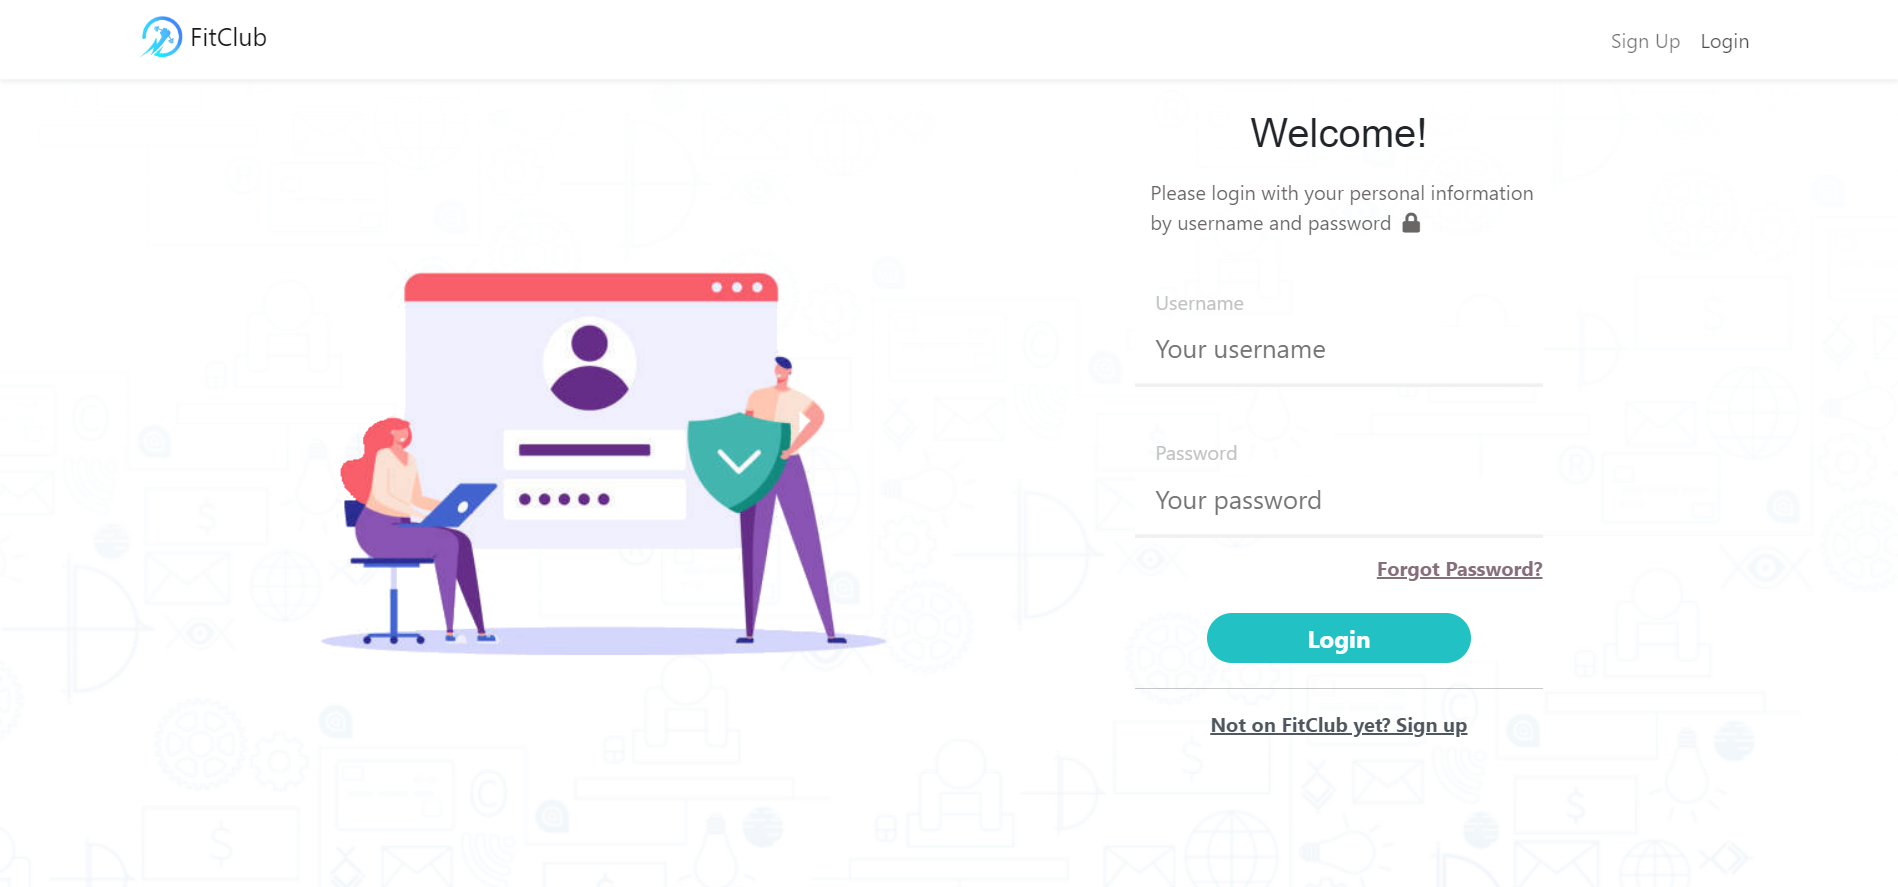
\includegraphics[width=13.8cm]{login-page.png}
		\caption{Pagina de autentificare}
	\end{center}
\end{figure}
\bigskip

\section{Înregistrarea}

Procedeul de înregistrare (Figura 4.2) a unui utilizator trebuie să respecte câteva reguli cu privire la informațiile furnizate, și anume:
\begin{itemize}
	\addtolength{\itemindent}{1cm}
	\item[$-$]Numele de utilizator trebuie să fie unic.
	\item[$-$]Atât numele de utilizator, cât și numele complet trebuie să aibă cel puțin 4 caractere, și maxim 255 caractere.
	\item[$-$]Parola trebuie să aibă cel putin 8 caractere, și să conțină cel puțin o literă mare, o literă mică, și un caracter special.
	\item[$-$]Adresa de email trebuie să fie unică pentru fiecare utilizator în parte și să aibă cel puțin 6 caractere și maxim 255 caractere.
	\newline
\end{itemize}

\begin{figure}[H]
	\begin{center}
		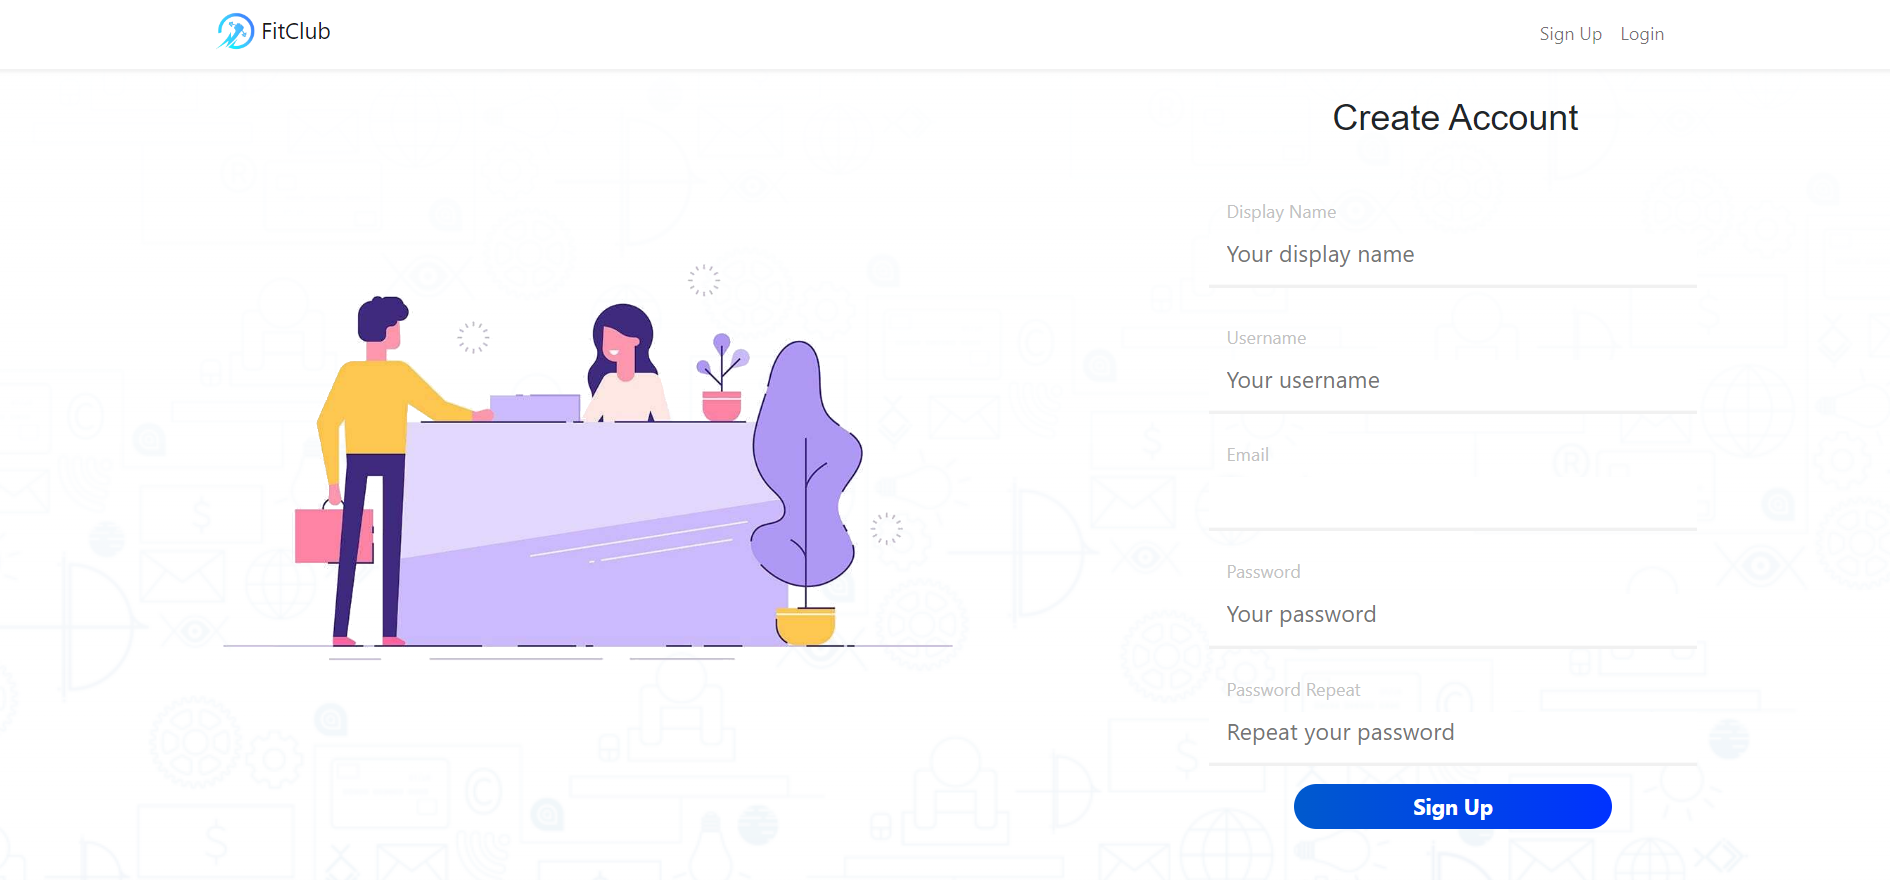
\includegraphics[width=13.8cm]{signup-page.png}
		\caption{Pagina de înregistrare}
	\end{center}
\end{figure}

Pentru a finaliza înregistrarea și a avea acces complet la resursele aplicației, utilizatorul trebuie să confirme adresa de email, accesând link-ul generat automat din cadrul mail-ului pe care îl va primi pe adresa furnizată în momentul înregistrării. (Figura 4.3)\newline 
\bigskip

\begin{figure}[H]
	\begin{center}
		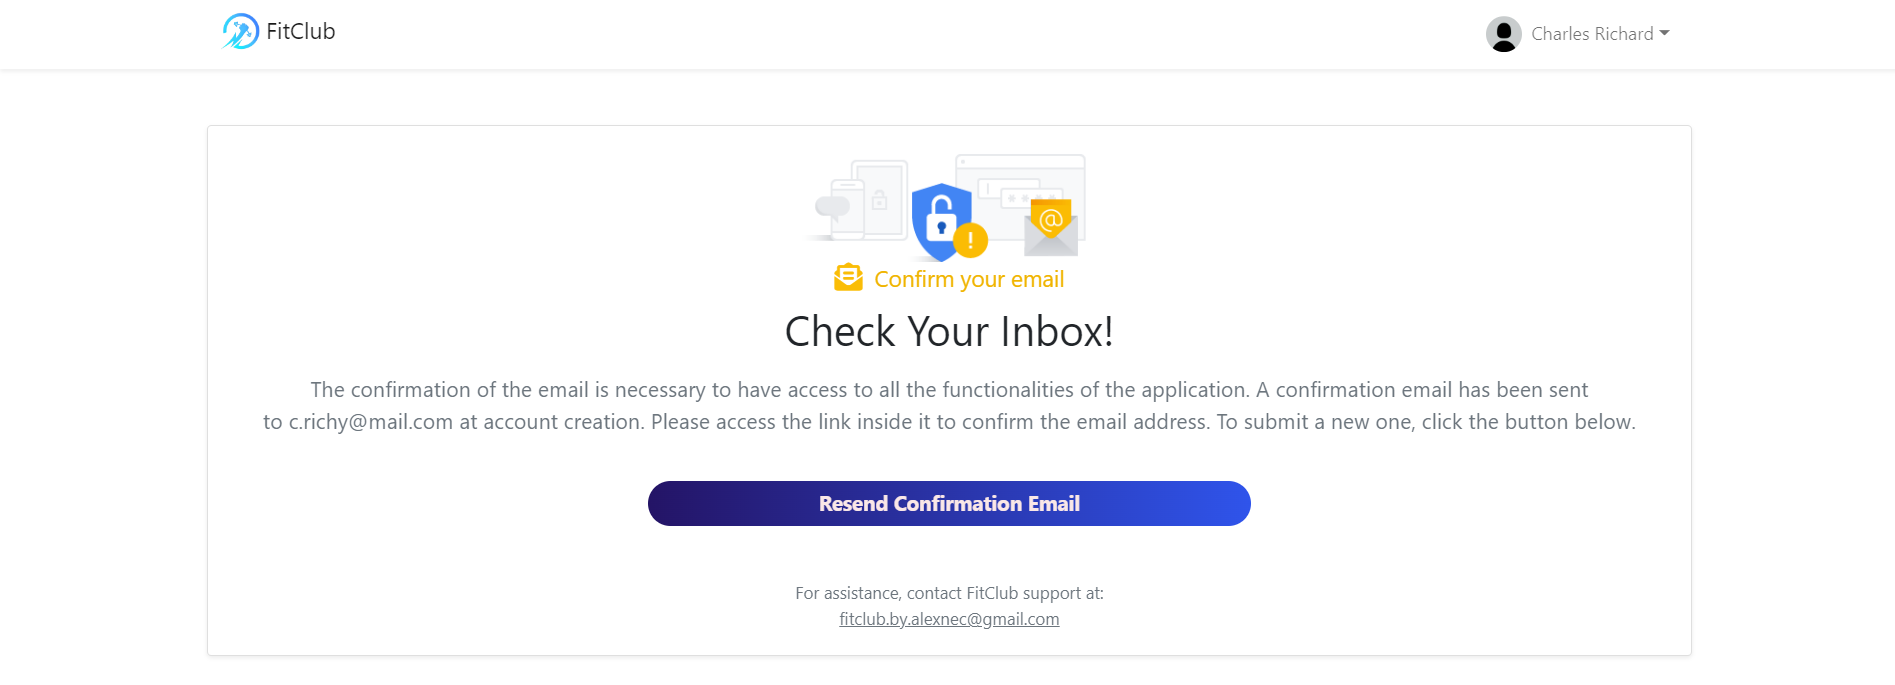
\includegraphics[width=13.8cm]{email-confirmation.png}
		\caption{Verificarea adresei de email pentru a finaliza înregistrarea}
	\end{center}
\end{figure}
\bigskip

De asemenea, autentificarea se va face automat după înregistrare, însă dacă utilizatorul nu reușește să își confirme adresa de email, atunci, din cauza securității aplicației, nu i se va permite să acceseze resursele disponibile.\newline

\textbf{Observație}: Link-ul transmis prin email este valid doar pentru 24 de ore de la momentul generării.\newline

În cazul în care utilizatorul nu a primit email-ul de confirmare sau acesta a accesat link-ul după ce a expirat, acesta poate solicita încă un email de confirmare care i se va trimite pe adresa furnizată în momentul înregistrării, cu aceeași valabilitate de 24 de ore (Figura 4.4).\newline
\bigskip

\begin{figure}[H]
	\begin{center}
		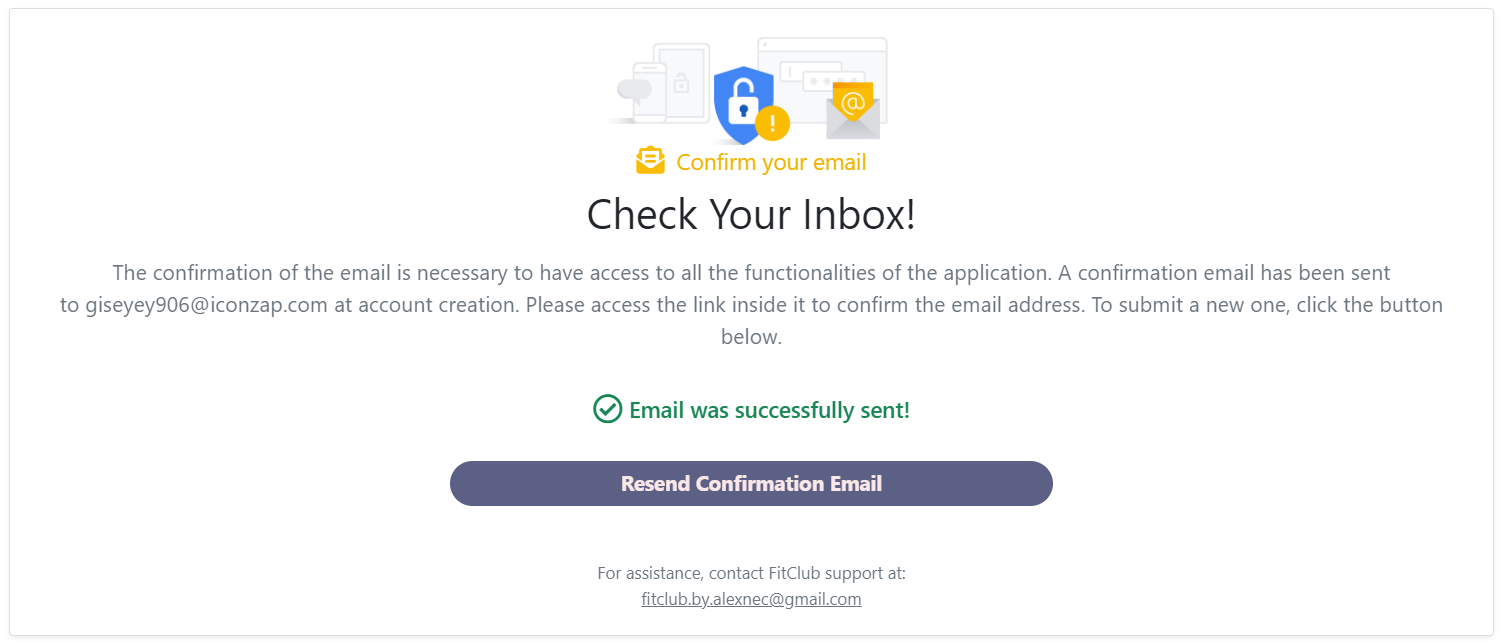
\includegraphics[width=13.8cm]{resend-email.png}
		\caption{Retrimiterea email-ului de confirmare}
	\end{center}
\end{figure}
\bigskip

Dacă procedeul de înregistrare se sfârșește cu succes, atunci utilizatorului i se va afișa pagina de confirmare (Figura 4.5), și va fi redirecționat în mod automat către pagina principală într-un interval de 5 secunde.\newline

De asemenea, odată ce această verificare a fost finalizată cu succes, nu va mai apărea în cadrul autentificărilor ulterioare.\newline
\bigskip

\begin{figure}[H]
	\begin{center}
		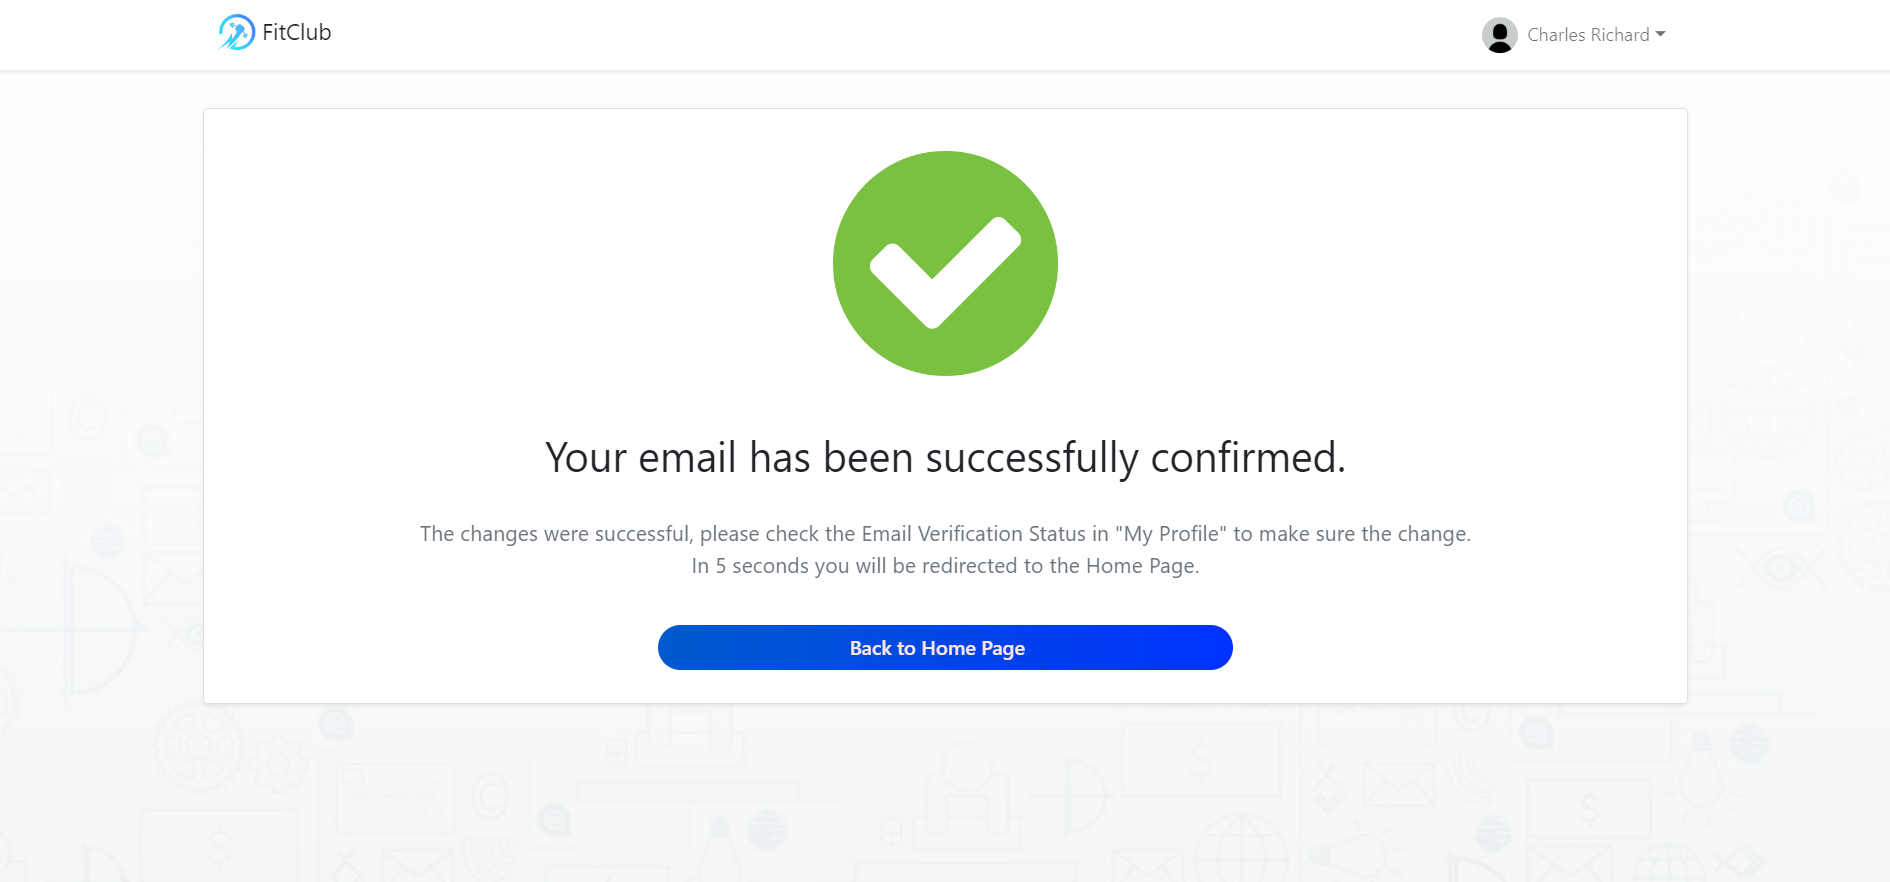
\includegraphics[width=13.8cm]{email-confirmed.png}
		\caption{Verificarea cu succes a adresei de email}
	\end{center}
\end{figure}
\bigskip

\section{Navigarea pe site}

Pagina principală în care apare fluxul de postări este determinat de postările celor pe care îi urmărește utilizatorul autentificat (Figura 4.6).\newline
 
Aplicația nu va include postări ale altor utilizatori în acest flux, nici în momentul încărcării postărilor vechi, și nici în momentul încărcării postărilor noi pe pagină.\newline

Utilizatorul are posibilitatea în cadrul acestei pagini de a adăuga o postare făcând click pe chenarul corespunzător unde este afișat indiciul de text: "Share something with your followers".\newline
\bigskip

\begin{figure}[H]
	\begin{center}
		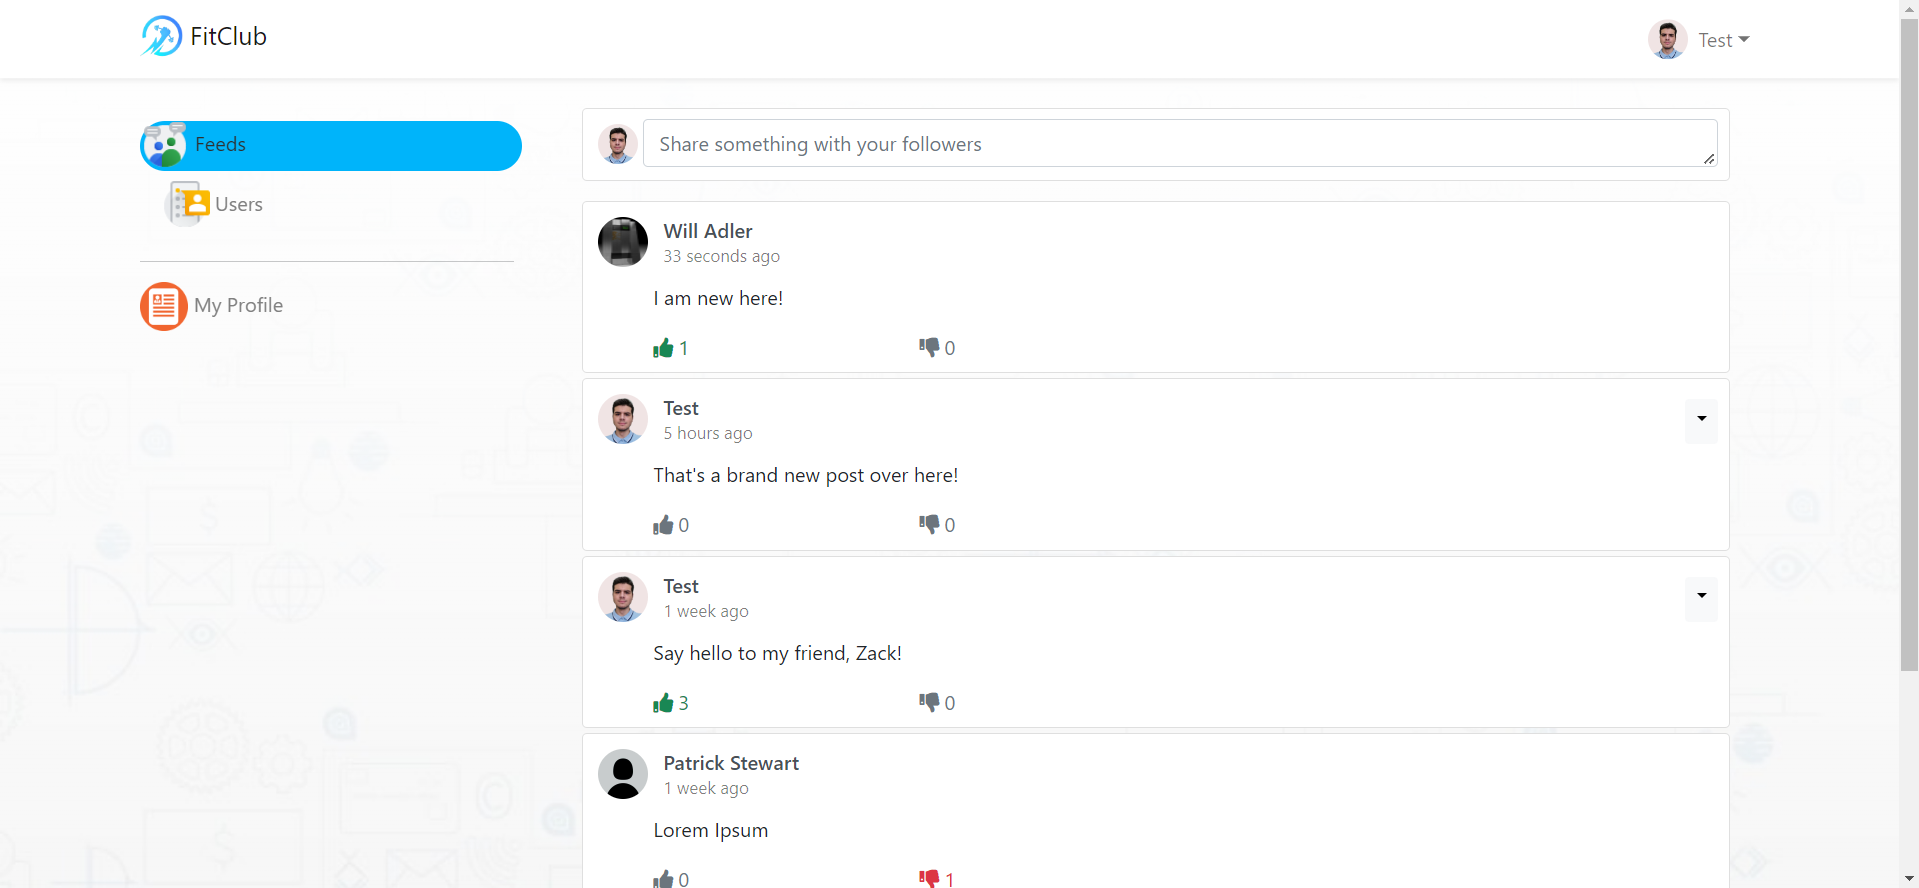
\includegraphics[width=13.8cm]{post-feed-ok.png}
		\caption{Fluxul de postări de pe pagina principală}
	\end{center}
\end{figure}

Atunci când chenarul este focalizat (Figura 4.7), utilizatorului i se vor afișa mai multe opțiuni, și anume să trimită postarea sau să o anuleze.\newline

De asemenea, acesta poate să încarce o imagine sau o animație (fișier cu extensia .gif), făcând click pe butonul "Choose file".\newline
\bigskip

\begin{figure}[H]
	\begin{center}
		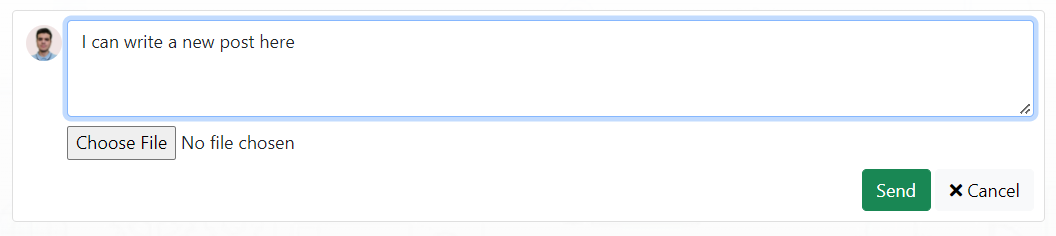
\includegraphics[width=13.8cm]{post-submit.png}
		\caption{Chenarul responsabil pentru scrierea propriu-zisă a postării}
	\end{center}
\end{figure}

Această imagine se va încărca în baza de date printr-o conversie în Base64, iar în momentul afișării pe pagină, aceasta va fi decodată corespunzător și afișată într-un format cât mai prietenos pentru a respecta raportul de aspect al container-ului postării (Figura 4.8).\newline
\bigskip

\begin{figure}[H]
	\begin{center}
		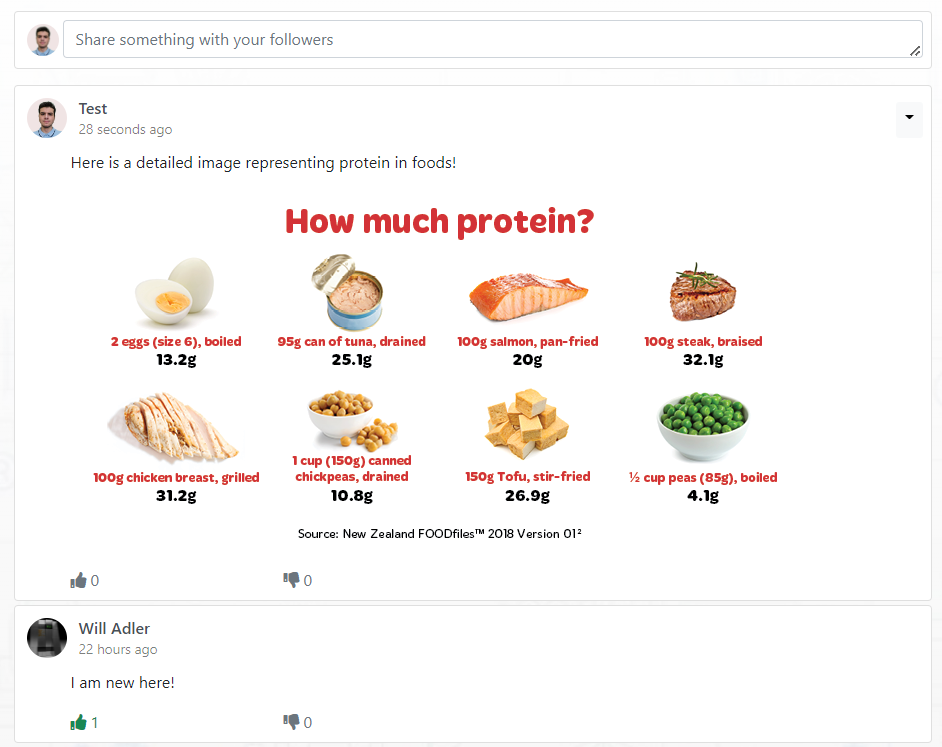
\includegraphics[width=12.9cm]{new-post-loaded.png}
		\caption{Fluxul de postări actualizat cu o postare având o imagine atașată}
	\end{center}
\end{figure}
\bigskip

De asemenea, în cadrul acestei pagini, utilizatorul poate reacționa la postările celor pe care îi urmărește. De exemplu, în Figura 4.8, se poate observa postarea utilizatorului cu numele "Will Adler", în care am reacționat printr-o apreciere.\newline

Pentru a demonstra, totodată, și funcționarea corectă a sistemului de reacții, vom schimba reacția acestei postări (Figura 4.9).\newline
\bigskip

\begin{figure}[H]
	\begin{center}
		
\includegraphics[width=12.9cm]{user-reaction.png}
		\caption{Modificarea reacției în cadrul unei postări}
	\end{center}
\end{figure}
\bigskip


Un utilizator autentificat poate să modifice anumite detalii direct de pe pagina sa de profil (Figura 4.10).\newline

În cadrul acestei pagini, i se va afișa și o confirmare a faptului că adresa sa de email a fost confirmată cu succes.\newline
Dacă acesta va opta în viitor să își modifice adresa de email, va fi nevoit să confirme și această adresă pentru a putea accesa în continuare site-ul, fără restricții.\newline
\bigskip

\begin{figure}[H]
	\begin{center}
		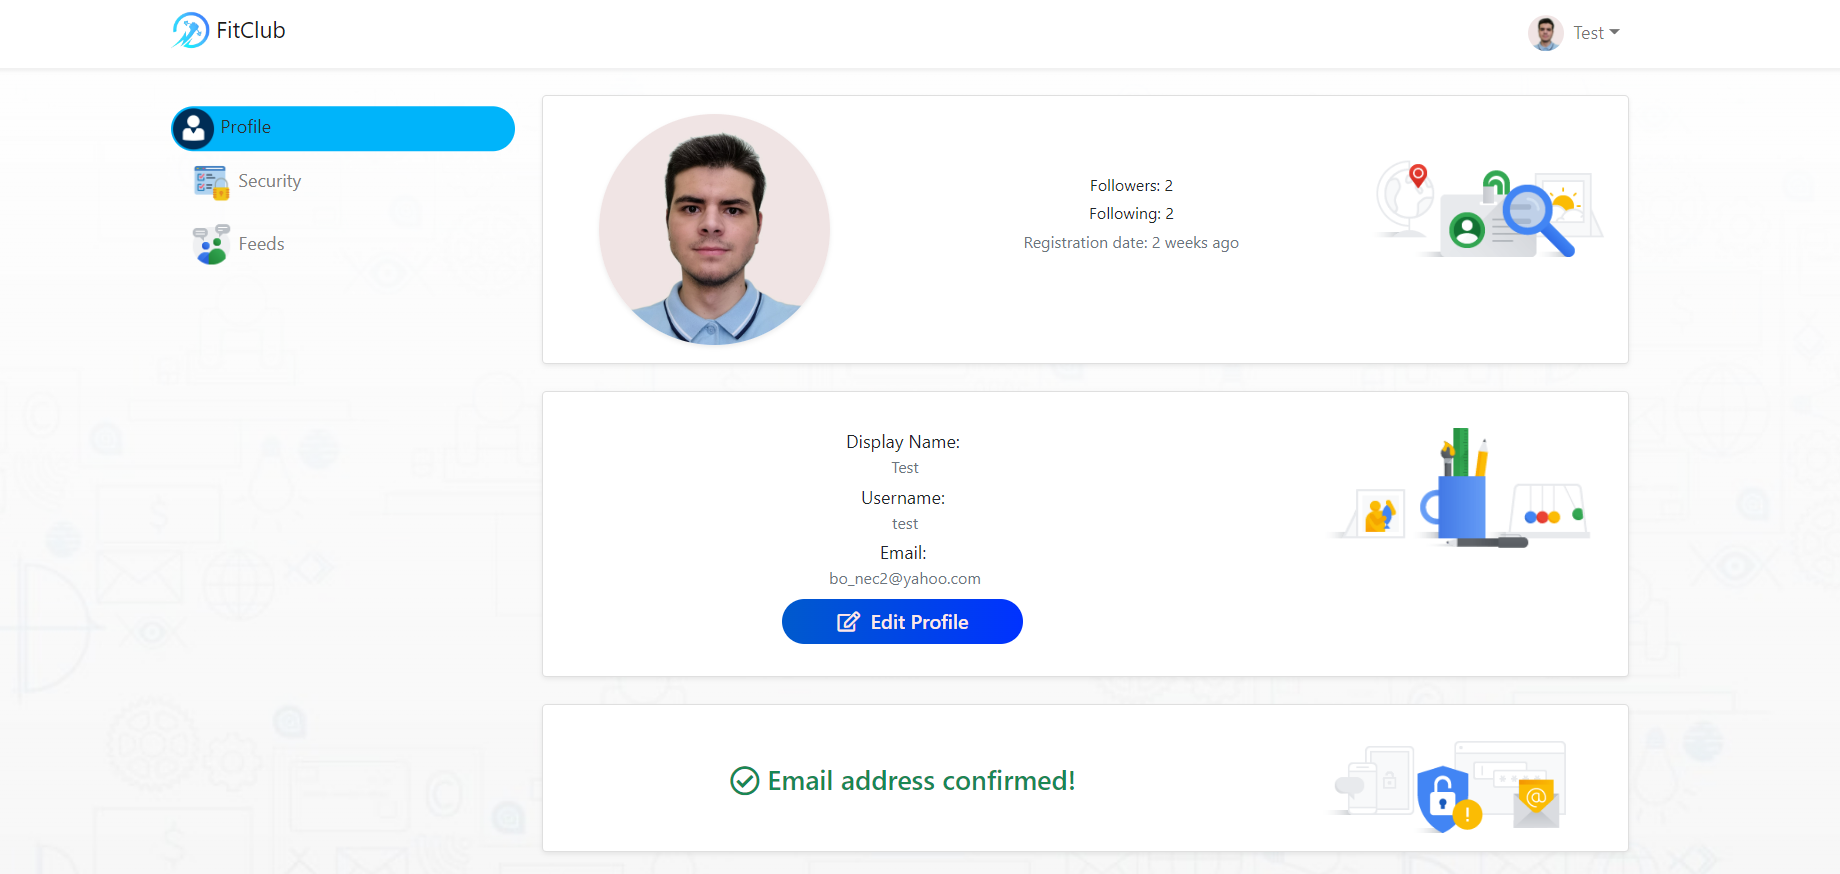
\includegraphics[width=13.7cm]{user-page.png}
		\caption{Pagina de profil a utilizatorului autentificat}
	\end{center}
\end{figure}
\bigskip

Utilizatorul poate să acceseze și o pagină responsabilă cu revizuirea credențialelor contului său (Figura 4.11). În cadrul acestei pagini, se va putea solicita schimbarea adresei de email, și respectiv a parolei.\newline

În ambele cazuri, înainte de a propaga orice schimbare legată de contul său în baza de date, utilizatorul va trebui să confirme că el acționează în scopul acestei schimbări prin accesarea link-ului inclus în mail-ul pe care îl va primi pe adresa de email confirmată în momentul înregistrării.\newline
\bigskip

\begin{figure}[H]
	\begin{center}
		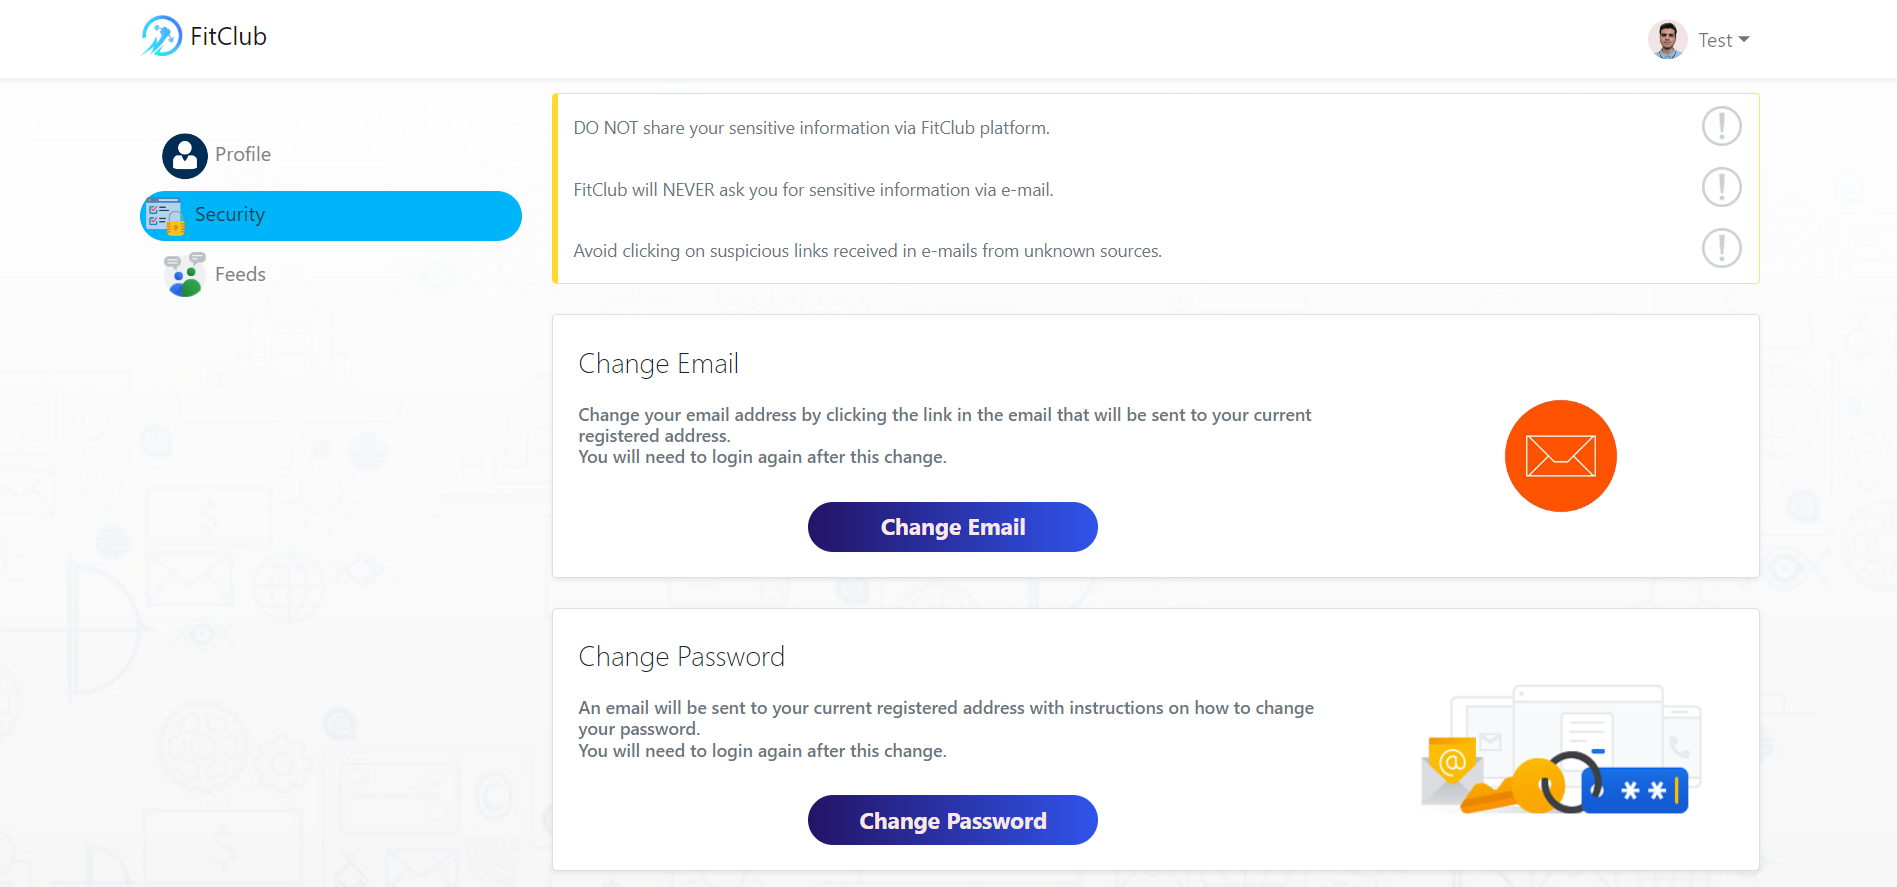
\includegraphics[width=13.7cm]{security-page.png}
		\caption{Pagina de unde se pot revizui credențialele de securitate}
	\end{center}
\end{figure}
\bigskip

Navigând către pagina de profil a oricărui utilizator, se pot vizualiza strict postările acestuia, și, de asemenea, sistemul de reacții funcționează și de pe această pagină (Figura 4.12).\newline
\bigskip

\begin{figure}[H]
	\begin{center}
		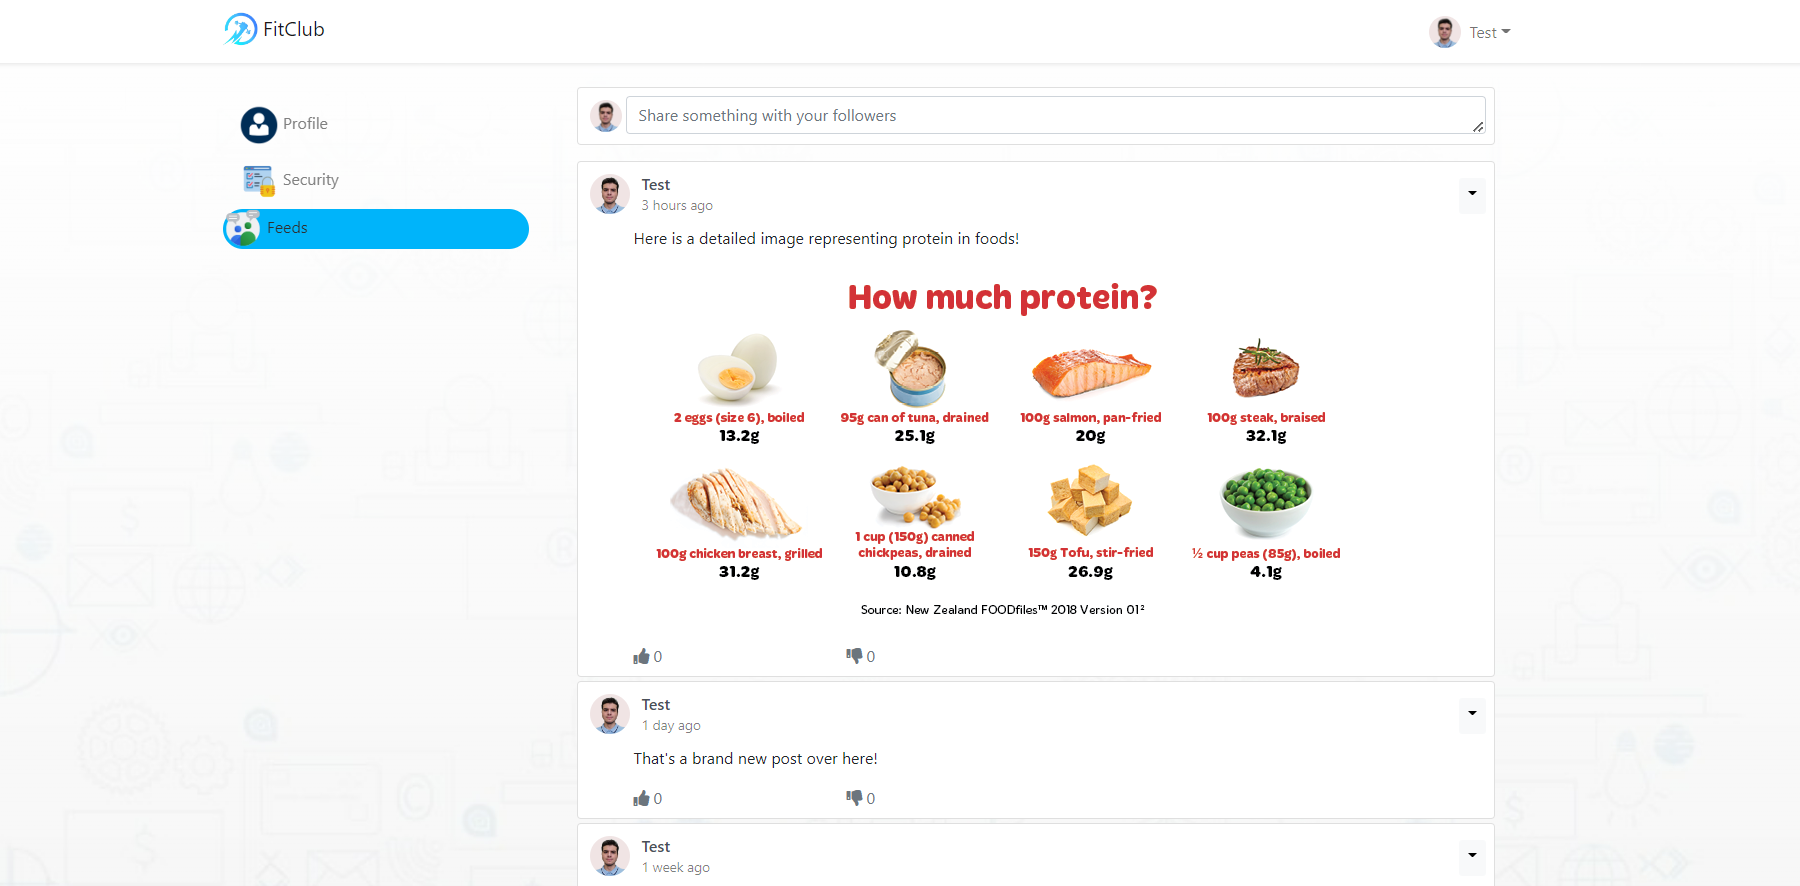
\includegraphics[width=13.7cm]{user-feeds.png}
		\caption{Postările de pe pagina de profil a unui utilizator}
	\end{center}
\end{figure}



\section{Accesarea nepermisă a aplicației}

Dacă un utilizator nu este autentificat, atunci acesta va putea să navigheze restricționat pe site, adică nu va putea să vizualizeze fluxul de postări de pe pagina principală, și nici postările specifice unui anumit utilizator (Figura 4.13).\newline
\bigskip

\begin{figure}[H]
	\begin{center}
		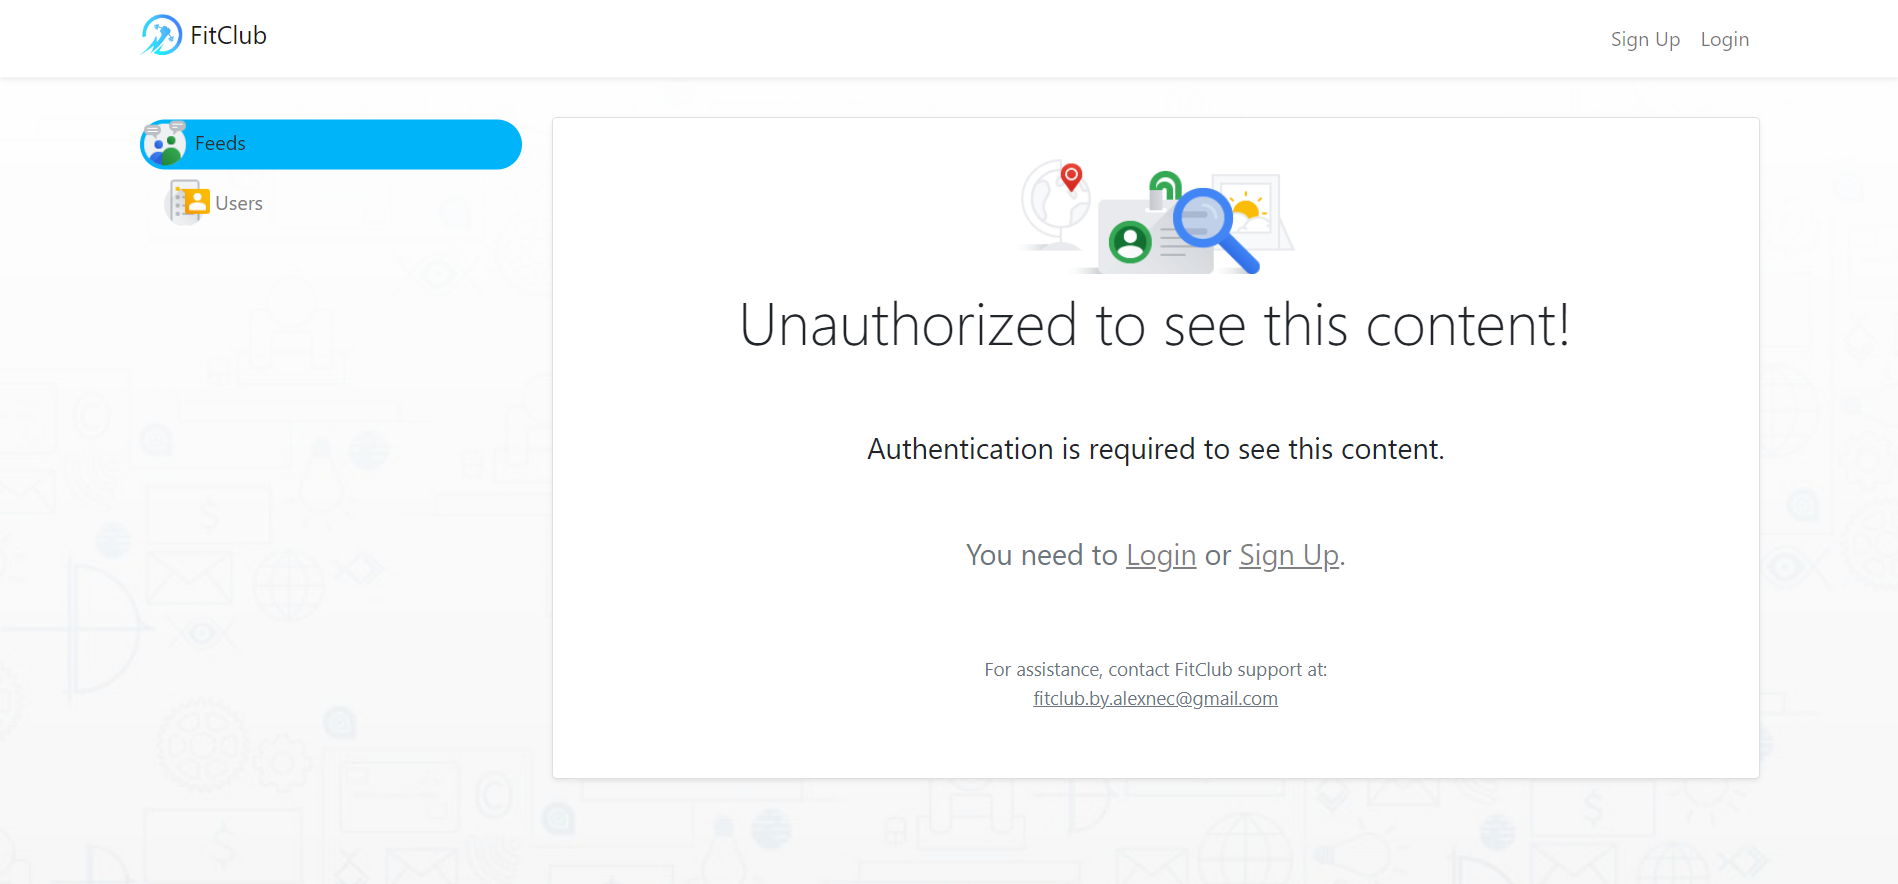
\includegraphics[width=13.1cm]{auth-required.png}
		\caption{Acces restricționat în cazul unui utilizator anonim}
	\end{center}
\end{figure}
\bigskip

Un utilizator anonim va putea să acceseze parțial paginile de profil ale utilizatorilor înregistrați pe site (Figura 4.14). Acest acces parțial se rezumă la posibilitatea de a vedea doar numele de utilizator, și respectiv, numele complet al unui utilizator.\newline
\bigskip

\begin{figure}[H]
	\begin{center}
		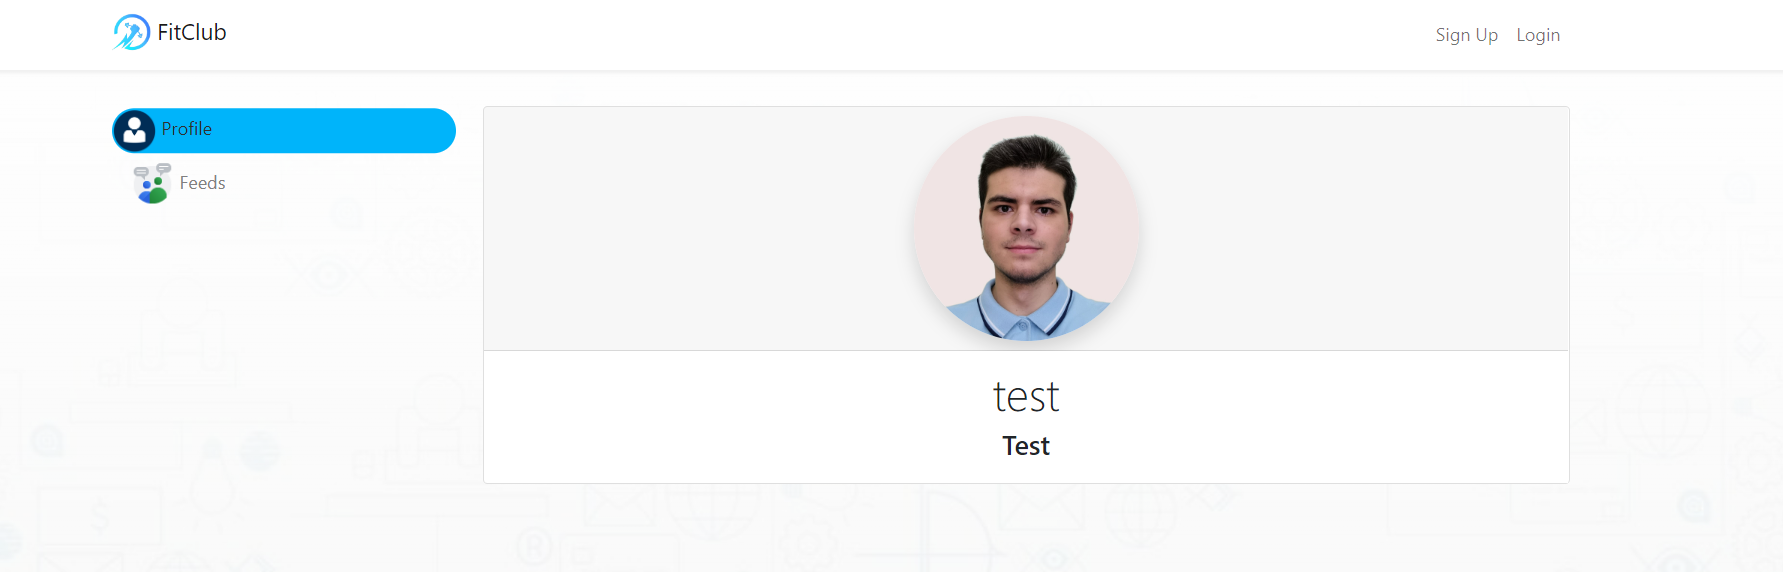
\includegraphics[width=12.3cm]{anonymous-user.png}
		\caption{Acces parțial la pagina de profil a unui utilizator}
	\end{center}
\end{figure}
\bigskip

De asemenea, același comportament este întâlnit și în cazul în care utilizatorul este autentificat, însă sesiunea acestuia expiră și este nevoit să se autentifice din nou pentru a obține un token valabil pentru încă 24 de ore (Figura 4.15).\newline

Chiar dacă utilizatorul este autentificat, și poate să intre în continuare pe pagina sa de profil, aplicația restricționează orice încercare de a face vreo schimbare referitoare la contul său, aplicația afișându-i un mesaj clar menit să-l îndrume pentru a putea dobândi din nou accesul.\newline
\bigskip

\begin{figure}[H]
	\begin{center}
		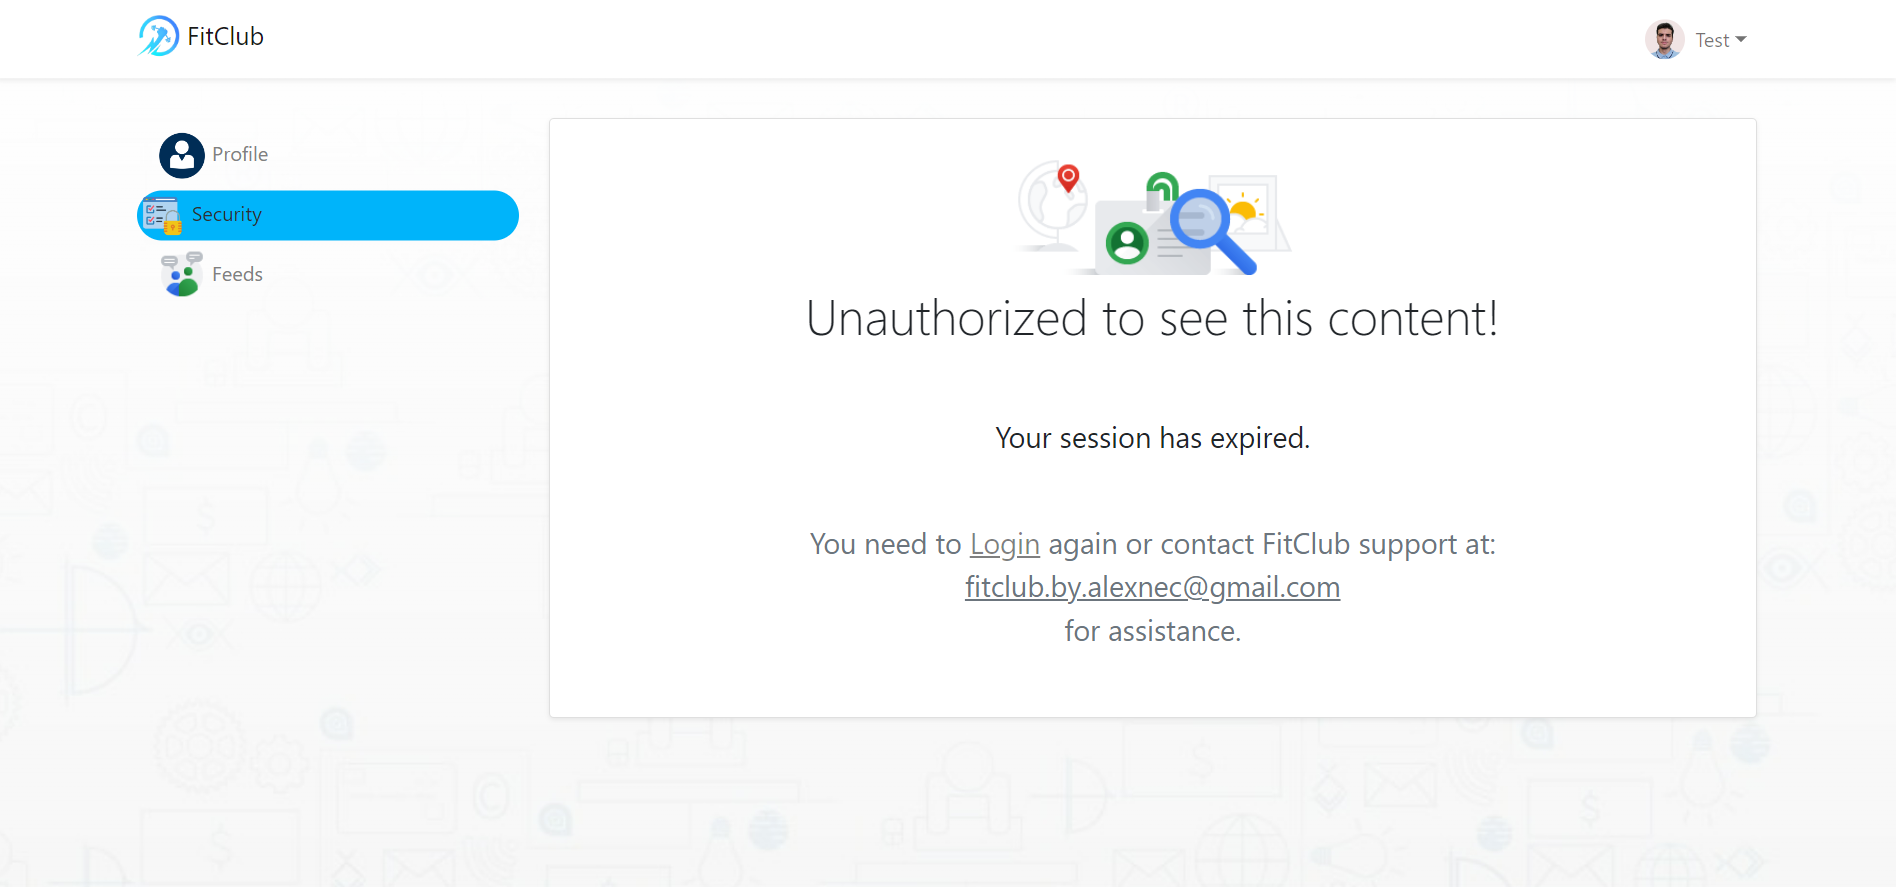
\includegraphics[width=13.8cm]{session-expired.png}
		\caption{Acces restricționat în cazul sesiunii expirate}
	\end{center}
\end{figure}

\label{chap:04}